\begin{center}
\Huge
	Funktioner	
\end{center}

\section*{Hvad er en funktion}
\stepcounter{section}

De eksempler på funktioner, vi indtil videre har stiftet bekendtskab med har været funktioner, vi har kunnet beskrive med en forskrift. Dette kunne være funktioner som $f(x) = 2x+3$, $g(x) = 5x^2$ eller $h(x) = \log_2(x)$. Vi kan bruge mængdebegrebet til at definere funktioner mere generelt, om end vi dog ikke vil definere funktionsbegrebet i sin fulde abstraktion. 

For en funktion $f$ definerer vi det, vi kalder for \textit{definitionsmængden} og \textit{værdimængden} for $f$.
\begin{defn}[Definitions- og værdimængde]
	For en funktion $f$ består definitionsmængden Dm($f$) af de $x$-værdier, vi kan anvende $f$ på.
	Værdimængden Vm($f$) består af alle de værdier, $f$ afbilder over i. Mere præcist
	\begin{align*}
		\{y  \mid  y = f(x) \textnormal{ for et } x \in \textnormal{Dm}(f)\}.
	\end{align*}
\end{defn}
Det vil ikke altid være klart, hvad værdimængden for en funktion er. Derfor skal vi bruge et begreb for den mængde, som en funktion $f$ antager værdier i. 
\begin{defn}[Dispositionsmængde]
	Dispositionsmængden for en funktion $f$ er den mængde, funktionen afbilder sine værdier ind i. Værdimængden 
	for $f$ er altså en delmængde af denne mængde. 
\end{defn}
For en funktion $f$ med definitionsmængde Dm$(f) = A$ og dispositionsmængde $B$ skriver vi ofte $f:A \to B$, når vi definerer funktionen. 
\begin{exa}
	Funktionen $f: \mathbb{R}_{\geq 0} \to \mathbb{R}_{\geq 0}$ givet ved
	\begin{align*}
		f(x) = \sqrt{x}
	\end{align*}
	kalder vi typisk for kvadratrodsfunktionen. 
	Funktionen $g:\mathbb{R} \to \mathbb{R}$ givet ved
	\begin{align*}
		g(x) = 2x + 3
	\end{align*}
	er en lineær funktion. 
\end{exa}
Sammenhængende delmængder af $\mathbb{R}$ kalder vi for intervaller. Et lukket interval fra $a$ til $b$ skrives $[a,b]$, og hvis $a$ og $b$ ikke er med i intervallet, skrives intervallet $]a,b[$ og intervallet kaldes åbent. 
I tilfældet af at kun $a$ er i intervallet, men ikke $b$ skrives $[a,b[$ og vice versa.
\begin{exa}
	På Figur \ref{fig:f1} ses grafen for en funktion $f$.
	\begin{figure}[H]
		\centering
		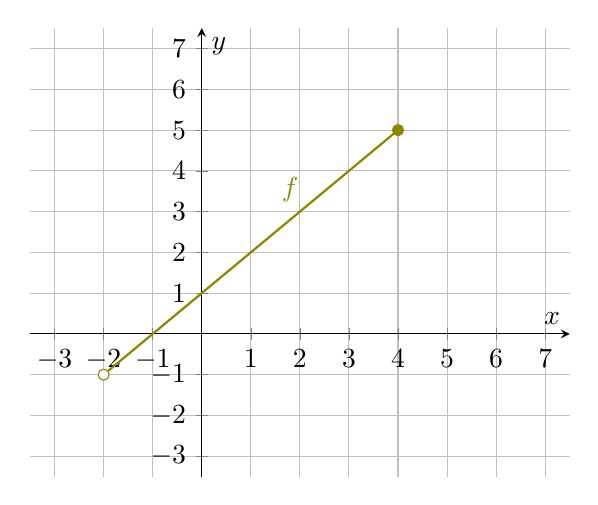
\begin{tikzpicture}
		\begin{axis}
		[axis lines = center, 
		xmin = -3.5, xmax = 7.5,
		ymin = -3.5, ymax = 7.5,
		grid = both,
		xtick = {-3,-2,...,6,7},
		ytick = {-3,-2,...,6,7},
		xlabel = $x$, 
		ylabel = $y$,	
		]
			\addplot[color = olive, thick, domain = -2:4] {x+1};	
			\filldraw[color = white](axis cs: -2,-1) circle (2pt);
			\filldraw[color = olive](axis cs: 4,5) circle (2pt);
			\draw[color = olive](axis cs: -2,-1) circle (2pt);
			\node[color = olive, anchor = south] at (axis cs: 1.8,3) {$f$};	
		\end{axis}
		\end{tikzpicture}
		\caption{Graf for funktionen $f$}
		\label{fig:f1}
	\end{figure}
	Vi kan se, at Dm$(f) = ]-2,4]$ og Vm$(f) = ]-1,5]$.
\end{exa}

Med begreberne defitionsmængde og værdimængde, kan vi nu definere en funktion lidt mere præcist.
\begin{defn}[Funktion]
	En funktion $f$ er en relation mellem Dm$(f)$ og Vm$(f)$, der relaterer ethvert element 
	$x\in \textnormal{Dm}(f)$ med et entydigt element $y \in \textnormal{Vm}(f)$ som $f(x) = y$. 
\end{defn}
Der må altså kun være én $y$-værdi til hver $x$-værdi, men der kan godt være flere $x$-værdier til samme $y$-værdi. (Som det eksempelvis er tilfældet med $f(x) = x^2.)$
\begin{exa}
	Vi lader $A$ betegne alle varer i et supermarked. Vi kan så definere en funktion
	$p:A \to \mathbb{R}$, der for enhver vare $x \in A$ giver os prisen på varen i kr. som $p(x)$. 
	Vi har fx. $p(\textnormal{Mælk}) = 14.75$ eller $p(\textnormal{Banan}) = 2.75$. Det er i dette tilfælde 
	ikke let at bestemme $\textnormal{Vm}(f)$, da vi så skal slå alle priserne i supermarkedet op. Vi skal 
	selvfølgelig have en entydig $y$-værdi for hver $x$-værdi, da én vare ikke kan have to forskellige priser.
\end{exa}
\begin{exa}\label{exa:udd}
Lad $U$ bestå af mængden af alle lange videregående uddannelser, og lad funktion $l:U \to \mathbb{R}$ være funktionen, der tager en uddannelse og giver gennemsnitsbruttoindkomsten efter afsluttet uddannelse. Så vil funktionen give os eksempelvis
\begin{align*}
l(\textnormal{Samfundsfag}) = 660.500.
\end{align*}
Værdimængden for denne funktion vil være
\begin{align*}
\textnormal{Vm}(l) = [267.200,1.383.200].
\end{align*}
\end{exa}

Vi kan også tænke på funktioner som diagrammer som set på Figur \ref{fig:diag}.
\begin{figure}[H]
	\centering
	\begin{tikzpicture}
		\draw[] (0,0) circle (1cm);
		\draw[] (4,0) circle (1cm);
		\node at (0,1.3) {$A$};
		\node at (4,1.3) {$B$};
		\draw[-{Stealth[scale = 1.3]}] (1.3,0) --(2.7,0);
		\node at (2,0.3) {$f$};
	\end{tikzpicture}
	\caption{Funktionsdiagram for funktionen $f$.}
	\label{fig:diag}
\end{figure}

\section*{Billede og urbillede}
Vi definerer \textit{billedet} og \textit{urbilledet} for mængder.
\begin{defn}[Billede og urbillede]
Lad $f:A \to B$ være en funktion, og lad $K\subseteq A$ være en delmængde af $A$. Så kalder vi mængden
\begin{align*}
f(K) = \{f(x) \mid x \in K\}
\end{align*}
for billedet af $K$ under $f$. 
Lad tilsvarende $L\subseteq B$. Så kaldes mængden 
\begin{align*}
 \{x \in A \mid f(x) \in K\}
\end{align*}
for urbilledet af $L$ under $f$.
\end{defn}

\begin{exa}
Lad $K = [1,2]\subseteq \mathbb{R}$, og lad $f:\mathbb{R} \to \mathbb{R}$ være givet ved
\begin{align*}
f(x) = 2x+1.
\end{align*}
Så er billedet af $K$ under $f$ givet ved mængden 
\begin{align*}
f([1,2]) = [3,5].
\end{align*}
Lader vi tilsvarende $L = [-2,0] \subseteq \mathbb{R}$, så vil urbilledet af $L$ under $f$ være givet ved mængden
\begin{align*}
[-1.5, -0.5].
\end{align*}
\end{exa}

Et diagram, der illustrerer billedet af en mængde under en funktion kan ses på Fig. \ref{fig:im}.
\begin{figure}[H]
	\centering
	\begin{tikzpicture}
		\draw[] (0,0) circle (1.5cm);
		\draw[] (6,0) circle (1.5cm);
		\node at (0,1.8) {$A$};
		\node at (6,1.8) {$B$};
		\draw[-{Stealth[scale = 1.3]}] (1.8,0) --(4.2,0);
		\node at (3,0.3) {$f$};
		\draw[] (0,0.6) circle (0.7cm);
		\node at (0,0.6) {$L$};
		\draw[] (6,0.6) circle (0.7cm);
		\node at (6,0.6) {$f(L)$};
		\draw[-{Stealth[scale = 1.3]}] (0.6,1.2) to[out = 45] (5.2,1.1);
		\node at (3,2.4) {$f$};
	\end{tikzpicture}
	\caption{Funktionsdiagram for funktionen $f$.}
	\label{fig:im}
\end{figure}


\newpage
\subsection*{Opgave 1}

Bestem defitionsmængde og værdimængde for følgende funktioner. 

\begin{center}
\resizebox{0.45\textwidth}{!}{
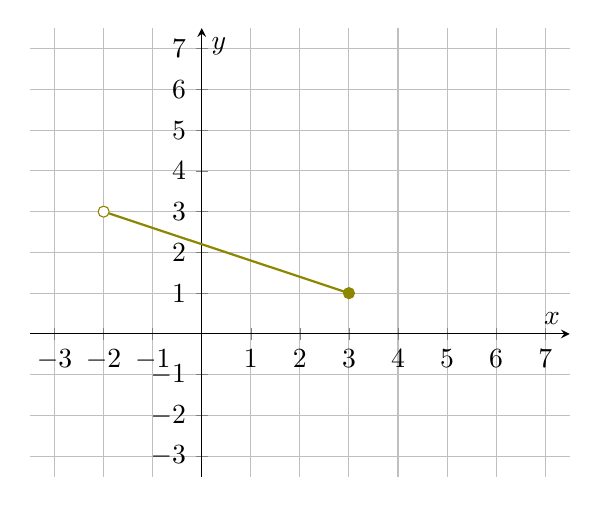
\begin{tikzpicture}
	\begin{axis}
	[axis lines = center, 
	xmin = -3.5, xmax = 7.5,
	ymin = -3.5, ymax = 7.5,
	grid = both,
	xtick = {-3,-2,...,6,7},
	ytick = {-3,-2,...,6,7},
	xlabel = $x$, ylabel = $y$
	]
		\addplot[color = olive, thick, domain = -2:3] {-2/5*x+2.2};	
		\filldraw[color = white](axis cs: -2,3) circle (2pt);
		\filldraw[color = olive](axis cs: 3,1) circle (2pt);
		\draw[color = olive](axis cs: -2,3) circle (2pt);
	\end{axis}
\end{tikzpicture}
}
\resizebox{0.45\textwidth}{!}{
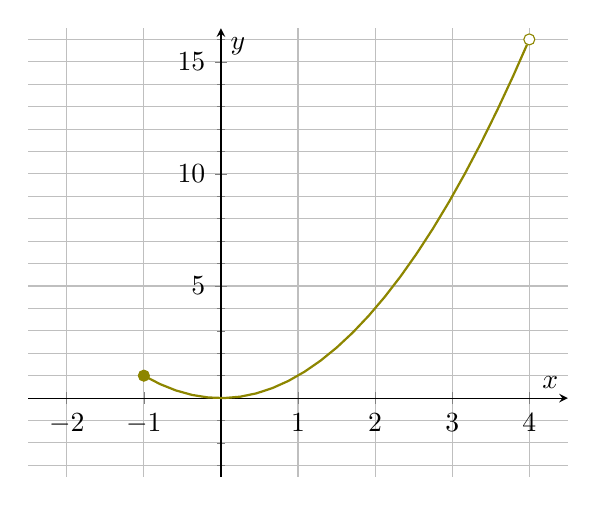
\begin{tikzpicture}
	\begin{axis}
	[axis lines = center, 
	xmin = -2.5, xmax = 4.5,
	ymin = -3.5, ymax = 16.5,
	xtick = {-3,-2,...,4,5},
	ytick = {-5,0,...,15,20},
	minor y tick num = 4,
	grid = both,
	xlabel = $x$, ylabel = $y$,
	]
		\addplot[color = olive, thick, domain = -1:4] {x^2};	
		\filldraw[color = white](axis cs: 4,16) circle (2pt);
		\filldraw[color = olive](axis cs: -1,1) circle (2pt);
		\draw[color = olive](axis cs: 4,16) circle (2pt);	
	\end{axis}
\end{tikzpicture}
}		
\resizebox{0.45\textwidth}{!}{
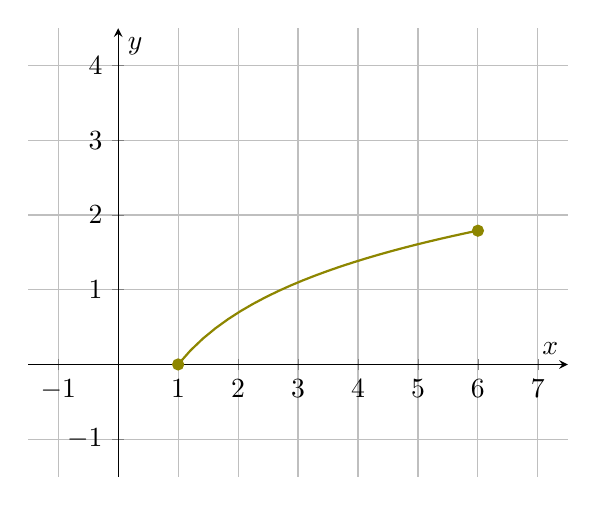
\begin{tikzpicture}
	\begin{axis}
	[axis lines = center, 
	xmin = -1.5, xmax = 7.5,
	ymin = -1.5, ymax = 4.5,
	grid = both,
	xtick = {-3,-2,...,6,7},
	ytick = {-3,-2,...,6,7},
	xlabel = $x$, ylabel = $y$
	]
		\addplot[color = olive, thick, domain = 1:6] {ln(x)};	
		\filldraw[color = olive](axis cs: 1,0) circle (2pt);
		\filldraw[color = olive](axis cs: 6, 1.79 ) circle (2pt);
	\end{axis}
\end{tikzpicture}
}
\resizebox{0.45\textwidth}{!}{
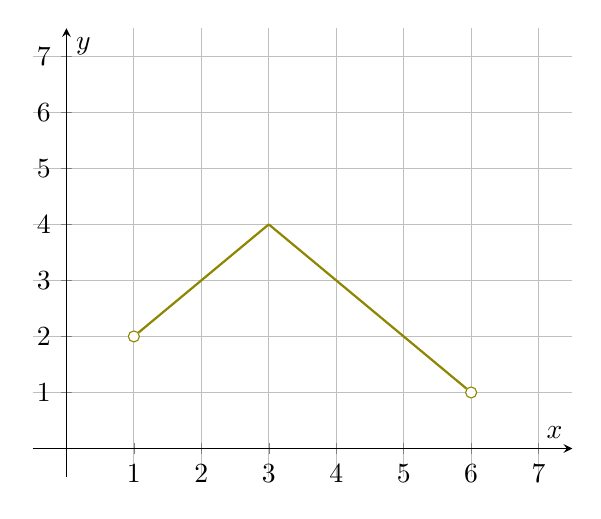
\begin{tikzpicture}
	\begin{axis}
	[axis lines = center, 
	xmin = -0.5, xmax = 7.5,
	ymin = -0.5, ymax = 7.5,
	grid = both,
	xtick = {-3,-2,...,6,7},
	ytick = {-3,-2,...,6,7},
	xlabel = $x$, ylabel = $y$
	]
		\addplot[color = olive, thick, domain = 1:3] {x + 1};
		\addplot[color = olive, thick, domain = 3:6] {-x + 7};	
		\filldraw[color = white](axis cs: 1,2) circle (2pt);
		\filldraw[color = white](axis cs: 6,1) circle (2pt);
		\draw[color = olive](axis cs: 1,2) circle (2pt);
		\draw[color = olive](axis cs: 6,1) circle (2pt);
	\end{axis}
\end{tikzpicture}
}
\resizebox{0.45\textwidth}{!}{
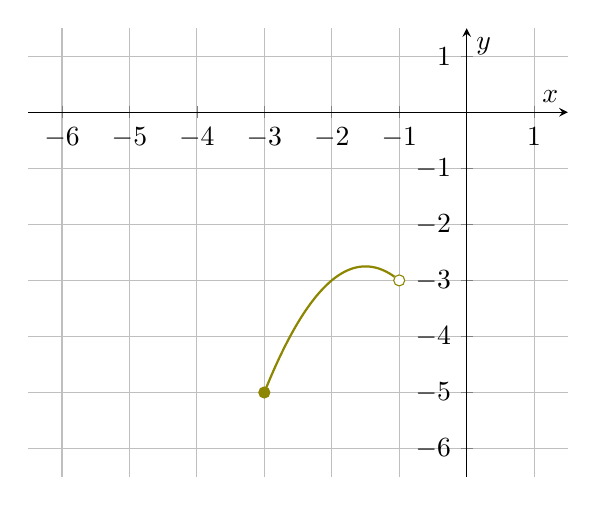
\begin{tikzpicture}
	\begin{axis}
	[axis lines = center, 
	xmin = -6.5, xmax = 1.5,
	ymin = -6.5, ymax = 1.5,
	grid = both,
	xtick = {-6,-5,...,6,7},
	ytick = {-6,-5,...,6,7},
	xlabel = $x$, ylabel = $y$
	]
		\addplot[color = olive, thick, domain = -3:-1, samples = 200] {-x^2-3*x-5};	
		\filldraw[color = white](axis cs: -1,-3) circle (2pt);
		\filldraw[color = olive](axis cs: -3,-5) circle (2pt);
		\draw[color = olive](axis cs: -1,-3) circle (2pt);
	\end{axis}
\end{tikzpicture}
}
\resizebox{0.45\textwidth}{!}{
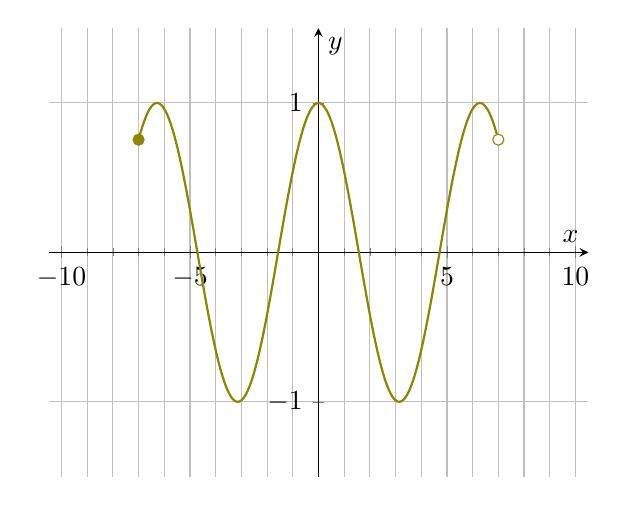
\begin{tikzpicture}
	\begin{axis}
	[axis lines = center, 
	xmin = -10.5, xmax = 10.5,
	ymin = -1.5, ymax = 1.5,
	grid = both,
	xtick = {-15,-10,...,10,15},
	minor x tick num = 4,
	ytick = {-1,0,1},
	xlabel = $x$, ylabel = $y$
	]
		\addplot[color = olive, thick, domain = -7:7, samples = 200] {cos(deg(x))};	
		\filldraw[color = white](axis cs: 7,0.754) circle (2pt);
		\filldraw[color = olive](axis cs: -7,0.754) circle (2pt);
		\draw[color = olive](axis cs: 7,0.754) circle (2pt);
	\end{axis}
\end{tikzpicture}
}
\end{center}

\subsection*{Opgave 2}
Bestem definitionsmængden og værdimængden for følgende funktioner ved evt. at tegne dem i Maple.
\begin{align*}
	&1) \ f(x) = \sqrt{x} & &2) f(x) = x^2 \\
	&3) \ f(x) = e^x & & 4) f(x) = \ln(x) \\
	&5) \ f(x) = \frac{1}{x}
\end{align*}

\subsection*{Opgave 3}
Bestem definitionsmængde og værdimængde for følgende funktioner.
\begin{align*}
	&1) \ f(x) = \sqrt{x-7} & &2) f(x) = x^2 - 10 \\
	&3) \ f(x) = \sqrt{-2x} & & 4) f(x) = \ln(4x - 20) \\
	&5) \ f(x) = \frac{1}{10x-70} & &6) f(x) = 2^x + 9
\end{align*}	


\subsection*{Opgave 4}
\begin{enumerate}
	\item Bestem værdimængden for funktionen $f:\mathbb{R} \to \mathbb{R}$ givet ved
	\begin{align*}
		f(x) = \lfloor x \rfloor,
	\end{align*}
	der runder alle tal ned til nærmeste heltal. 
\end{enumerate}

\subsection*{Opgave 5}
\begin{enumerate}[label=\roman*)]
\item Lad $f:\mathbb{R} \to \mathbb{R}$ være givet ved
\begin{align*}
f(x) = x + 4.
\end{align*}
Bestem billedet af følgende delmængder af $\mathbb{R}$ under $f$:
\begin{align*}
&1) \ \{1,2,4\} &&2) \ [0,5]\\
&3) \ \emptyset &&4) \ \{20\}
\end{align*}
\item Lad $f: \mathbb{R} \to \mathbb{R}$ være givet ved 
\begin{align*}
f(x) = 2x^2-4x+1.
\end{align*}
Bestem billedet af følgende delmængder af $\mathbb{R}$ under $f$ (det kan være en fordel at plotte $f$):
\begin{align*}
&1)\  [3,8] &&2) \  \{1,\hdots, 8\};\\
&3)\  \emptyset &&4)\ [-2,2];
\end{align*}
\item Lad $f:\mathbb{R} \to \mathbb{Z}$ være givet ved
\begin{align*}
f(x) = \lceil x \rceil + 2.
\end{align*}
Bestem billedet af følgende delmængder af $\mathbb{R}$ under $f$:
\begin{align*}
&1) \ [-4,5]  &&2) \ \{1.1,1.2,1.3,1.7,1.85\}\\
&3) \ [0,1]  &&4) \ \{1,2,3,4\}\\
\end{align*}
\end{enumerate}

\subsection*{Opgave 6}
Lad $l$ være funktionen fra Eksempel \ref{exa:udd}. Bestem billedet af mængden 
\begin{align*}
\{\textnormal{Medicin, Tandlæge, Erhvervsøkonomi}\}.
\end{align*}
Lønstatistik kan findes \href{https://cepos.dk/artikler/se-listen-hvilke-uddannelser-giver-den-hoejeste-indkomst/}{\color{blue!60} her}.

\subsection*{Opgave 7}
\begin{enumerate}[label=\roman*)]
\item Lad $f: \mathbb{R} \to \mathbb{R}$ være givet ved 
\begin{align*}
	f(x) = x-5.
\end{align*}
Bestem urbilledet af følgende mængder under $f$:
\begin{align*}
	&1) \  [9,12] &&2) \ \{2\}\\
	&3) \ \{-4,-2,-1\} &&4) \ \emptyset
\end{align*}

\item Lad $f:\mathbb{R}_{\geq 0} \to \mathbb{R}_{\geq 0}$ være givet ved
\begin{align*}
	f(x) = \sqrt{x}.
\end{align*}
Bestem urbilledet af følgende mængder under $f$:
\begin{align*}
	&1) \ \{2\}  &&2) \  [0,4] \\
	&3) \ \{1,3,4,5,6\} &&4) \ [8,16] 
\end{align*}

\item Lad $l$ være funktionen fra Eksempel \ref{exa:udd}. Bestem urbilledet af mængden $[700.000,1.000.000]$.
\end{enumerate}
